\chapter{Backend}\label{ch:A}
\section{Microservices}
Our backend designed in microservice architecture. In this section we will describe advantages and disadvantages of that approach
	\subsection{Pros}
		\subsubsection{Load handling}
		Each microservice has own resources. It means we can control which of them is going to have most computational power and distribute resources depending on the service's needs
		\subsubsection{Developing}
		Developing a new microservice is always easy, because all other services, except the one which is being developed, can be developed independently. Team's work is parallel. So the development stage is shorter
		\subsubsection{Database}
		Microservices has own database, so access is not limited for whole system. In monolith access to database is limited to number of database replicas and connection pool and whole system is limited by that. In microservices we have the same limitations, but only for microservice.
	\subsection{Cons}
		\subsubsection{Integration}
		As we said, mircoservices are good with databases, but in case we need to move data across services, it becomes a problem. Microservices' internal communication becomes a problem for system's network. Also, requests' idempotency becomes a problem, so we have to use message brockers to guarantee a recieve by another service. If we some data on different microservices are related, we will need to guarantee data's consistency, for us it means, we will load network with another bunch of requests between services
		\subsubsection{Bug tracking}
		If some service uses a lot of other services, it becomes hard to track bugs and handle them through all services. In such cases it is good to have some logger, which will collect logs from services and show us.
		\subsubsection{Refactoring}
		When we refactor microservices and change data representation or communication protocols, we should be ready for other services to be unable to communicate with current one
\section{Authorization}
	\subsection{JWT}
	In project we are using JWT (JSON Web Token). Token is divided on three parts by dot.
	\begin{itemize}
		\item Header
		\item Payload
		\item Signature
	\end{itemize}
	
	Structure: \textbf{xxx.yyy.zzz}
	
	\subsubsection{Header}
	The header typically consists of two parts: the type of the token, which is JWT, and the signing algorithm being used, such as HMAC SHA256 or RSA (For example see Figure \ref{fig:header}). Then, this JSON is Base64Url encoded to form the first part of the JWT.
	
	
		
	
	
	
	\subsubsection{Payload}
	The second part of the token is the payload, which contains the claims. Claims are statements about an entity (typically, the user) and additional data (For example see Figure \ref{fig:payload}). There are three types of claims: registered, public, and private claims. The payload is then Base64Url encoded to form the second part of the JSON Web Token.
	
		\paragraph{Registered claims}
		These are a set of predefined claims which are not mandatory but recommended, to provide a set of useful, interoperable claims. Some of them are: iss (issuer), exp (expiration time), sub (subject), aud (audience), and others.
		\paragraph{Public claims}
		These can be defined at will by those using JWTs. But to avoid collisions they should be defined in the IANA JSON Web Token Registry or be defined as a URI that contains a collision resistant namespace.
		\paragraph{Private claims}
		These are the custom claims created to share information between parties that agree on using them and are neither registered or public claims.
		
		
	\subsubsection{Signature}
	To create the signature part you have to take the encoded header, the encoded payload, a secret, the algorithm specified in the header, and sign that.
	
	The signature is used to verify the message wasn't changed along the way, and, in the case of tokens signed with a private key, it can also verify that the sender of the JWT is who it says it is.
	
	
		\begin{figure}[h!]
    		\centering
    		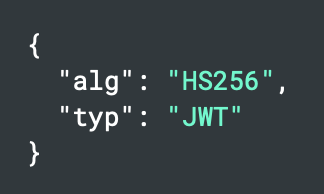
\includegraphics{header.png}
    		\caption{Header}
    		\label{fig:header}
		\end{figure}
	
		\begin{figure}[h!]
    		\centering
    		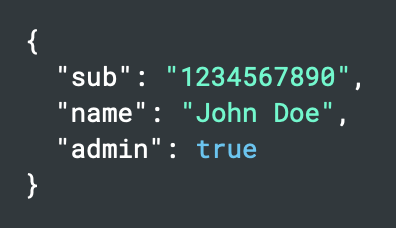
\includegraphics{payload.png}
    		\caption{Payload}
    		\label{fig:payload}
		\end{figure}
		
		
	\subsubsection{Summary}
	The output is three Base64-URL strings separated by dots that can be easily passed in HTML and HTTP environments, so we can easily transfer information like user id, and permissions through this token, and be sure data verified, because it is signed.
	
	\subsection{Implementation}
	In our project we developed an authorization service which will sign tokens and refresh them. Also we have verification middleware on each service, so we can be sure token is valid and not expired.
	
		When user credentials passed to server it hashes it and compares to hash we have in database for this user. We keep no plain text passwords and hash functions can't be reversed, so they can not be leaked. In case everything okay it returns token string.
		
		We are using jwt-go package to sign token.
		
	
\section{Database}
	For our project we chose Postgres database because we are familiar with it, also it is open source, that's why we can use it for free.
	
	SQL databases provide fast data access and data modification. We are not going to delete often or change table structure, so there is no need to use collection based databases like Mongo.
	
\section{Maze generation}
	